% ============================================================
%  ICD-10 Clinical Codification — Project Report
%  NLP-I  |  UAB  |  2025-2026
% ============================================================
\documentclass[10pt,a4paper,twocolumn]{article}

% ---- Encoding & Fonts ----
\usepackage[T1]{fontenc}
\usepackage[utf8]{inputenc}
\usepackage{lmodern}

% ---- Page Geometry ----
\usepackage[a4paper, top=2cm, bottom=2cm, left=1.8cm, right=1.8cm, columnsep=0.6cm]{geometry}

% ---- Mathematics ----
\usepackage{amsmath,amssymb}

% ---- Graphics & Figures ----
\usepackage{graphicx}
\usepackage{float}

% ---- Tables ----
\usepackage{booktabs}
\usepackage{array}

% ---- Code (verbatim fallback — no listings needed) ----
\usepackage{verbatim}

% ---- Paragraph spacing ----
\setlength{\parskip}{6pt}
\setlength{\parindent}{0pt}

% ============================================================
\begin{document}

% ---- Title (full-width, above two columns) ----
\twocolumn[
  \begin{@twocolumnfalse}
    \centering
    {\LARGE\bfseries ICD-10 Clinical Codification:\\[6pt]
     A Deep Learning Pipeline for Spanish Clinical Text Classification\par}
    \vspace{0.6cm}
    {\large NLP-I --- Natural Language Processing I\par}
    {\large Universitat Aut\`onoma de Barcelona,\; Q2 / 2025--2026\par}
    \vspace{0.3cm}
    {\small\itshape Kaggle: \texttt{uab-asho-ai-codification} \quad
     Instructors: Ernest Valveny \& Lei Kang \quad \today\par}
    \vspace{0.8cm}

% ---- Abstract (still inside \twocolumn[...], so full-width) ----
    \begin{abstract}
    We present an end-to-end deep learning pipeline for automated ICD-10
    codification of Spanish clinical report literals. The task is formulated as
    single-label multiclass classification over 36 categories (digits
    \texttt{0}--\texttt{9} and letters \texttt{A}--\texttt{Z}), mapping short,
    noisy clinical notes to their corresponding first-character ICD-10 category.
    Starting from a provided baseline that achieved \textbf{56--57\%} accuracy
    using standard RoBERTa with CLS/Mean pooling, we designed an optimized
    architecture featuring: (i) a domain-specific Spanish biomedical pre-trained
    backbone, (ii) a custom Attention Pooling layer, (iii) Multi-Sample Dropout
    regularization, (iv) ICD-10 dictionary augmentation with a strict
    split-before-augment protocol, (v) encoder layer freezing, and (vi) balanced
    class-weight cross-entropy loss. Our final optimized pipeline achieved
    \textbf{80.4\%} validation accuracy and \textbf{71.8\%} macro-F1, together
    with a \textbf{79.2\%} score on the Kaggle public leaderboard ---
    a relative improvement of $+42\%$ in accuracy and $+178\%$ in macro-F1
    with respect to the mean-pooling baseline.
    \end{abstract}
    \vspace{0.6cm}
  \end{@twocolumnfalse}
]

% ============================================================
\section{Introduction}
\label{sec:intro}
% ============================================================

The International Classification of Diseases (ICD) is the global standard for
encoding clinical diagnoses, maintained by the World Health Organization. Assigning
ICD codes to health-related documents, commonly known as \textit{ICD coding}, is
an essential operation in hospital administration, epidemiological surveillance,
and insurance reimbursement. In its tenth revision (ICD-10), the code space spans
more than 70\,000 unique codes, organized hierarchically by chapter, section, and
category.

Manual coding is performed by trained professional coders who read electronic
medical records (EMRs) and assign the most appropriate code. This process is
labor-intensive, error-prone, and costly: a report by the US Centers for Medicare
and Medicaid estimated a 6.8\% coding error rate in 2000, with the annual cost of
incorrect coding reaching US\$25 billion [1]. Automation of this task has therefore
attracted considerable academic interest over the past three decades.

\subsection{Task Formulation}

This project addresses a constrained but practically important sub-task of full
ICD-10 coding, as defined by the UAB--ASHO competition [2]:

\begin{itemize}
  \item \textbf{Input:} A single clinical report literal from
        \texttt{codification\_data.csv} (training) or
        \texttt{leaderboard\_data.csv} (test). Literals are brief --- typically
        2--3 words --- and frequently contain medical abbreviations, Catalan/Spanish
        bilingual expressions, and non-standard spellings.
  \item \textbf{Output:} A single ICD-10 category label defined as the first
        character of the full ICD-10 code:
        \begin{equation}
          y_{\text{category}} = \texttt{Code}[0].\text{upper()}
        \end{equation}
        For example, \texttt{Code = "I420"} $\Rightarrow$ \texttt{y\_category = "I"};
        \texttt{Code = "3E03329"} $\Rightarrow$ \texttt{y\_category = "3"}.
  \item \textbf{Classes:} 36 categories: $[\texttt{0}, \texttt{1}, \ldots, \texttt{9},
        \texttt{A}, \texttt{B}, \ldots, \texttt{Z}]$. Ten categories (\texttt{0}--\texttt{9})
        correspond to ICD-10-PCS (Procedure Coding System), and 26 categories
        (\texttt{A}--\texttt{Z}) correspond to ICD-10-CM (Clinical Modification)
        diagnostic categories.
\end{itemize}

\subsection{Challenges}

The dataset presents three intertwined machine learning challenges:

\begin{enumerate}
  \item \textbf{Severe Class Imbalance.} The training data is dominated by a
        handful of common categories such as \texttt{Z} (factors influencing
        health), \texttt{O} (pregnancy, childbirth), and \texttt{0} (surgical
        procedures), while long-tail categories such as \texttt{U} or \texttt{W}
        contain only a handful of samples. A naive model predicting only the
        top-3 categories can already exceed 60\% accuracy --- making raw accuracy a
        misleading metric.

  \item \textbf{Domain and Lexical Mismatch.} Two data sources with fundamentally
        different vocabularies are available:
        \begin{itemize}
          \item \textbf{Primary dataset} (\texttt{codification\_data.csv}):
                13\,702 raw clinical report literals in colloquial
                Catalan/Spanish, containing misspellings, abbreviations
                (e.g.\ \textit{HTA}, \textit{IRC}), and single-word diagnoses.
          \item \textbf{Augmentation dataset} (\texttt{icd\_d\_p\_pairs.csv}):
                Formal, clean ICD-10 dictionary descriptions (e.g.\ \textit{``C\'{o}lera
                debido a Vibrio cholerae O1, biotipo cl\'{a}sico''}), averaging
                $\sim$35 words per entry.
        \end{itemize}
        Naive concatenation of both sources would introduce distribution shift
        into the validation set if the split is performed after augmentation.

  \item \textbf{Short Literal Lengths.} Real clinical reports average only 2--3
        words and peak at 9 words. This severely limits the contextual signal
        available to the encoder, making disambiguation (e.g.\ \textit{ia}
        = \textit{Insufici\`encia A\`ortica} vs.\ \textit{Inseminaci\'{o}
        Artificial}) almost impossible without domain-specific pre-training.
\end{enumerate}

% ============================================================
\section{Related Work}
\label{sec:related}
% ============================================================

Automated ICD coding has evolved through three major paradigms, as surveyed
comprehensively by Yan et al.\ [1].

\paragraph{Rule-based methods (1990s--2000s).}
Early systems extracted coding rules from ICD guidelines and converted them into
executable if-else logical programs [3]. On the small CCHMC radiology dataset
(45 codes), these approaches achieved up to 90.26\% training accuracy. However,
they fail to scale: as code count grows, rule conflicts multiply and portability
to new hospital systems is negligible.

\paragraph{Traditional machine learning (2000s--2015).}
Feature-engineering approaches using TF-IDF and n-gram features fed into SVM,
logistic regression, or random forest classifiers became the standard. Perotte
et al.\ [4] proposed Flat and Hierarchy-based SVMs using TF-IDF features on
MIMIC-III, achieving modest results. These methods train an independent binary
classifier per ICD code and do not capture inter-code relationships or sparse
clinical semantics.

\paragraph{Deep learning (2015--present).}
Neural network-based methods now dominate the field. Key milestones include:
\begin{itemize}
  \item \textbf{CNN + label-wise attention (CAML/DR-CAML)} [5]:
        achieved Micro-F1 of 0.457/0.529 on MIMIC-II/MIMIC-III-Full.
  \item \textbf{Hierarchical RNN (HA-GRU)} [6]: two-level GRU encoding to
        handle long EMR documents.
  \item \textbf{Graph Neural Networks (HyperCore, MSResGCN)}: exploit the
        ICD taxonomy tree structure via GCN to model code co-occurrence and
        inheritance relationships.
  \item \textbf{Pre-trained Language Models (BioBERT, ClinicalBERT,
        PubMedBERT)} [7, 8]: domain-specific BERT variants trained on biomedical
        corpora. The top LAAT/JointLAAT model [9] achieved Macro-F1 of 0.107
        and Micro-F1 of 0.575 on MIMIC-III-Full.
\end{itemize}

A key lesson from the PLM-based literature is that standard general-purpose
multilingual models underperform on clinical text due to domain-specific
vocabulary, and that the 512-token limit poses challenges for long EMR documents.
In our task, the \textit{short} literal length actually plays in favour of
transformer models, as truncation is not an issue --- motivating our choice of
a Spanish biomedical RoBERTa backbone.

For Spanish clinical NLP specifically, the \textbf{CodiEsp} shared task
(CLEF eHealth 2020) [10] provides the closest public benchmark: 1\,000 Spanish
EMRs, averaging 397 tokens each and labeled with Spanish ICD-10-CM/PCS codes
at the full-code level. Our task is a simplified, first-character variant using
much shorter (2--9 token) literals from Catalan hospital records.

% ============================================================
\section{Proposed Solution}
\label{sec:method}
% ============================================================

Our pipeline was developed in two stages: a baseline reproducing the instructor's
reference system, followed by a fully optimized architecture. Both share the same
backbone model.

\subsection{Pre-trained Backbone}

The backbone model is \texttt{PlanTL-GOB-ES/roberta-base-biomedical-clinical-es},
a RoBERTa-base architecture [11] pre-trained on more than 1 billion tokens of
Spanish biomedical and clinical text, including:

\begin{itemize}
  \item Clinical case reports and discharge summaries.
  \item SciELO biomedical publications.
  \item Spanish medical registries, patents (EMEA), and PubMed abstracts.
  \item Wikipedia life-sciences articles.
\end{itemize}

Key architectural parameters of the backbone are summarized in
Table~\ref{tab:backbone}.

\begin{table}[H]
\centering
\caption{Architecture parameters of the backbone model.}
\label{tab:backbone}
\begin{tabular}{ll}
\toprule
\textbf{Parameter} & \textbf{Value} \\
\midrule
Architecture type    & RoBERTa-base \\
Transformer layers   & 12 \\
Hidden feature size  & 768 \\
Attention heads      & 12 \\
Feed-forward size    & 3072 \\
Total parameters     & 126M \\
\bottomrule
\end{tabular}
\end{table}

Standard multilingual models (e.g.\ mBERT) are pre-trained primarily on Wikipedia
and lack representations for Spanish medical abbreviations such as \textit{HTA}
(hypertension), \textit{IRC} (chronic renal failure), or \textit{VHC} (hepatitis
C virus). The domain-specific backbone provides pre-built subword embeddings for
these clinical forms, enabling fine-tuning to converge faster and to more
clinically meaningful representations.

\subsection{Text Preprocessing}

The preprocessing pipeline is intentionally lightweight, preserving the
information content of the original clinical text so that the biomedical
tokenizer can extract its pre-trained subword representations:

\begin{equation}
  x_{\text{clean}} = \mathrm{RegExSub}\!\left(\mathrm{Strip}\!\left(\mathrm{String}(x_{\text{raw}})\right),\; \texttt{\textbackslash s+},\; \texttt{' '}\right)
\end{equation}

Crucially, we do \emph{not} apply:
\begin{itemize}
  \item Lowercasing --- the case distinction between \texttt{I} (circulatory) and
        \texttt{i} is clinically meaningful.
  \item Accent removal --- Spanish/Catalan accents are semantically discriminative
        (e.g.\ \textit{c\'{o}lera} vs.\ \textit{colera}).
  \item Punctuation stripping --- punctuation is part of the biomedical vocabulary.
\end{itemize}

\subsection{Data Augmentation --- Split-Before-Augment Protocol}

To address severe class imbalance in long-tail categories, we augment the
training set using formal ICD-10 dictionary entries from
\texttt{icd\_d\_p\_pairs.csv}. This file contains official code--description
pairs that provide clean, lexically rich supervision for each category.

A critical design decision is the \textbf{split-before-augment protocol}: the
primary clinical dataset is first split stratified into training and validation
subsets, and augmentation data is appended \emph{only} to the training split.
This prevents dictionary entries from appearing in or inflating the validation set,
which would produce an overoptimistic accuracy estimate. The pipeline is:

\begin{enumerate}
  \item Load 13\,702 primary clinical literals.
  \item Perform stratified 80/20 split: \textbf{10\,961 train} / \textbf{2\,741 val}.
  \item Sample up to 1\,000 augmentation entries per class from
        \texttt{icd\_d\_p\_pairs.csv}.
  \item Concatenate augmentation with train split only.
\end{enumerate}

\subsection{Tokenization}

Sequences are tokenized using the backbone's BPE tokenizer. The maximum sequence
length was empirically optimized to $L = 64$ tokens: an analysis of the primary
dataset revealed that the longest clinical literal spans only 49 subword tokens.
Setting $L = 64$ (instead of the baseline's 128) halves the GPU memory footprint
of the attention matrices and accelerates training with zero information loss.

\subsection{Model Architecture}

The complete classification model, implemented as the \texttt{ICD10Classifier}
PyTorch module, processes each clinical literal through the following stages:

\paragraph{1. Transformer Encoder.}
The tokenized input (IDs + attention mask) is passed through the frozen or
fine-tuned layers of the backbone, yielding a sequence of hidden states
$\mathbf{H} \in \mathbb{R}^{B \times L \times d}$, where $B$ is the batch size,
$L$ is the sequence length, and $d = 768$ is the hidden dimension.

\paragraph{2. Attention Pooling.}
Instead of CLS or mean pooling, we apply a learned \textbf{Attention Pooling}
layer that computes a weighted sum of token hidden states, concentrating on
clinically relevant terms:

\begin{align}
  e_i &= \mathbf{w}_2^\top \tanh(\mathbf{W}_1 \mathbf{h}_i) \in \mathbb{R}, \quad i=1,\ldots,L \\
  e_i &\leftarrow -\infty \quad \text{if token } i \text{ is a padding token} \\
  \alpha_i &= \frac{\exp(e_i)}{\sum_{j=1}^{L} \exp(e_j)} \\
  \mathbf{v} &= \sum_{i=1}^{L} \alpha_i\, \mathbf{h}_i \in \mathbb{R}^d
\end{align}

where $\mathbf{W}_1 \in \mathbb{R}^{d \times d}$ and
$\mathbf{w}_2 \in \mathbb{R}^{d}$ are learnable parameters. Masking padding
tokens with $-\infty$ before softmax ensures that they receive zero weight in
the final aggregation. This mechanism allows the model to dynamically focus
on core clinical nouns (e.g.\ \textit{bronquial}, \textit{dilatada}) while
downweighting grammatical function words.

\paragraph{3. Multi-Sample Dropout.}
To combat overfitting on the small primary clinical dataset, the pooled
representation $\mathbf{v}$ is passed through $K=5$ parallel dropout layers
with probability $p=0.15$. The final logits are the average across all $K$
forward passes:

\begin{equation}
  \hat{\mathbf{y}} = \frac{1}{K} \sum_{k=1}^{K} \left( \mathbf{W}_c \cdot \mathrm{Dropout}_k(\mathbf{v}) + \mathbf{b}_c \right)
\end{equation}

This acts as a mini-ensemble at the forward pass level, forcing the classifier
weights to remain robust to different subsets of features being zeroed out. It
accelerates convergence and reduces variance in the final predictions without
increasing inference cost.

\paragraph{4. Linear Classification Head.}
A linear projection maps the averaged $768$-dimensional representation to $36$
class logits: $\mathbf{W}_c \in \mathbb{R}^{36 \times 768}$, initialized with
Xavier uniform initialization.

The complete forward pass is summarized in Table~\ref{tab:forward}.

\begin{table}[H]
\centering
\caption{Forward pass of \texttt{ICD10Classifier} showing tensor shapes at each stage
($B$ = batch size).}
\label{tab:forward}
\begin{tabular}{ll}
\toprule
\textbf{Stage} & \textbf{Output Shape} \\
\midrule
BPE Tokenization ($L=64$)                    & $B \times 64$ \\
RoBERTa Encoder (12 layers, $d=768$)         & $B \times 64 \times 768$ \\
Attention Pooling (learned weights)          & $B \times 768$ \\
Multi-Sample Dropout ($K=5$, $p=0.15$)      & $5 \times B \times 768$ \\
Linear Head ($768 \to 36$) + Average         & $B \times 36$ \\
Cross-entropy loss $+$ argmax                & $B \times 1$ \\
\bottomrule
\end{tabular}
\end{table}

\subsection{Encoder Layer Freezing}

To prevent catastrophic forgetting of Spanish clinical representations and to
reduce the number of trainable parameters (from 126M to $\approx$43.7M), the
following parts of the encoder are frozen:

\begin{itemize}
  \item Token, position, and type embedding layers.
  \item Transformer encoder layers 0--5 (bottom half).
\end{itemize}

Only the top 6 transformer layers, the attention pooling weights, and the
classification head are updated during backpropagation. This also serves as
an implicit regularizer and significantly accelerates each training epoch on
the available consumer-grade GPU hardware (NVIDIA RTX 3050 6 GB).

\subsection{Training Configuration}

\paragraph{Optimizer.}
AdamW [12] is used for all trainable parameters with learning rate
$\eta = 2 \times 10^{-5}$ and weight decay $\lambda = 0.01$.

\paragraph{Learning Rate Schedule.}
A cosine decay schedule with a 10\% linear warmup is applied over the full
training horizon. This allows the model to adapt its learning rate from the
initial unstable phase to a stable decay, which is critical when fine-tuning
pre-trained transformers.

\paragraph{Effective Batch Size.}
Due to VRAM constraints (6 GB laptop GPU), we use a physical batch size of 32
and accumulate gradients over 4 steps, yielding an effective batch size of 128.
Large effective batch sizes stabilize gradient estimates on highly imbalanced
targets [13].

\paragraph{Loss Function.}
We use the weighted cross-entropy loss with balanced class weights $w_c$
computed via sklearn's \texttt{compute\_class\_weight("balanced")}:
\begin{equation}
  w_c = \frac{N}{C \cdot N_c}
\end{equation}
where $N$ is the total number of training samples, $C = 36$ is the number of
classes, and $N_c$ is the sample count of class $c$. This prevents frequent
classes such as \texttt{Z} and \texttt{O} from dominating gradient updates and
forces the model to learn representations for the rare long-tail categories.

\paragraph{Early Stopping.}
The model checkpoint with the highest \textbf{Macro-F1} on the validation set is
saved. Training terminates if the Macro-F1 does not improve for 10 consecutive
epochs (patience = 10), with a maximum of 50 epochs.

\paragraph{Automatic Mixed Precision.}
All forward and backward passes use \texttt{torch.float16} (AMP) with a
\texttt{GradScaler}, halving memory usage and accelerating matrix multiplications
on CUDA tensor cores. Gradient clipping with \texttt{max\_norm=1.0} prevents
numerical instability from the scaled gradients.

% ============================================================
\section{Experiments and Evaluation}
\label{sec:experiments}
% ============================================================

\subsection{Dataset Statistics}

Table~\ref{tab:dataset} summarizes the characteristics of both data sources.

\begin{table*}[t]
\centering
\caption{Dataset statistics.}
\label{tab:dataset}
\begin{tabular}{lll}
\toprule
\textbf{Property} & \textbf{Primary (Clinical)} & \textbf{Augmentation (ICD Dict.)} \\
\midrule
File                     & \texttt{codification\_data.csv} & \texttt{icd\_d\_p\_pairs.csv} \\
Total samples            & 13\,702                         & $>$1\,000\,000 pairs \\
Avg.\ literal length     & 2--3 words                      & $\sim$35 words \\
Max.\ literal length     & 9 words / 49 subwords           & $\sim$140 subwords \\
Language                 & Spanish / Catalan mix           & Formal Spanish \\
Text quality             & Raw, noisy, abbreviated         & Clean, structured \\
Number of classes        & 36                              & 36 \\
\bottomrule
\end{tabular}
\end{table*}

\subsection{Hyperparameter Configurations}

Table~\ref{tab:hyperparameters} presents the full configuration comparison
between the instructor-provided baseline and our optimized pipeline.

\begin{table*}[t]
\centering
\caption{Hyperparameter configurations for baseline and optimized models.}
\label{tab:hyperparameters}
\begin{tabular}{lp{6cm}p{6cm}}
\toprule
\textbf{Hyperparameter} & \textbf{Baseline} & \textbf{Optimized (Ours)} \\
\midrule
Backbone & \texttt{roberta-base-biomedical-clinical-es} & \texttt{roberta-base-biomedical-clinical-es} \\
Pooling strategy & CLS token / Mean & Custom Attention Pooling \\
Max sequence length $L$ & 128 & 64 \\
Augmentation data & None & \texttt{icd\_d\_p\_pairs.csv} ($\leq$1000/class) \\
Encoder layers frozen & None (all 12 active) & Embeddings + layers 0--5 \\
Multi-Sample Dropout & Single Dropout($p$=0.10) & 5$\times$ Dropout($p$=0.15) \\
Physical batch size & 128 & 32 \\
Gradient accumulation steps & None & 4 \\
Effective batch size & 128 & 128 \\
Learning rate & $2 \times 10^{-5}$ & $2 \times 10^{-5}$ \\
Weight decay & 0.01 & 0.01 \\
Warmup ratio & 10\% & 10\% \\
LR schedule & Cosine with warmup & Cosine with warmup \\
Loss function & Standard CrossEntropy & Balanced Class-Weighted CrossEntropy \\
Early stopping metric & Validation Accuracy & Validation Macro-F1 \\
Early stopping patience & 10 epochs & 10 epochs \\
Max training epochs & 50 & 50 \\
\bottomrule
\end{tabular}
\end{table*}

\subsection{Evaluation Metrics}

We evaluate models using three complementary metrics:

\begin{itemize}
  \item \textbf{Validation Loss:} Cross-entropy loss on the held-out validation
        set. Lower is better.
  \item \textbf{Validation Accuracy:} Fraction of correctly classified literals.
        This is the Kaggle leaderboard metric but is misleading when classes are
        imbalanced.
  \item \textbf{Validation Macro-F1:} The unweighted average of per-class F1
        scores:
        \begin{equation}
          \text{Macro-F1} = \frac{1}{C} \sum_{c=1}^{C} F1_c, \qquad F1_c = \frac{2 \cdot P_c \cdot R_c}{P_c + R_c}
        \end{equation}
        Macro-F1 gives equal weight to all 36 classes, making it sensitive to
        performance on rare diagnostic categories. This is our \emph{primary}
        optimization and model selection metric, as a model that ignores rare
        classes would be clinically harmful.
\end{itemize}

\paragraph{Why Accuracy is Insufficient.}
Because the primary training set is heavily imbalanced (categories \texttt{Z},
\texttt{O}, and \texttt{0} alone account for more than 60\% of samples), a
degenerate model predicting only these three classes would achieve over 60\%
accuracy while completely failing on the remaining 33 clinical categories. In
a real clinical deployment, such systematic misclassifications would lead to
incorrect administrative records, billing errors, and potentially compromised
patient care.

% ============================================================
\section{Results}
\label{sec:results}
% ============================================================

\subsection{Model Performance Comparison}

Table~\ref{tab:results} presents the complete performance comparison across all
model configurations evaluated on the clean stratified validation split and on
the Kaggle public leaderboard.

\begin{table*}[t]
\centering
\caption{Model performance comparison on clinical codification. Best values in \textbf{bold}.}
\label{tab:results}
\begin{tabular}{lcccc}
\toprule
\textbf{Pipeline Architecture} & \textbf{Val.\ Loss} & \textbf{Val.\ Acc.} & \textbf{Val.\ Macro-F1} & \textbf{Kaggle Acc.} \\
\midrule
Baseline: RoBERTa + CLS Pooling                        & 1.724 & 0.565 & 0.245 & 0.558 \\
Baseline: RoBERTa + Mean Pooling                       & 1.682 & 0.570 & 0.258 & 0.562 \\
RoBERTa + Att.\ Pool + Multi-Dropout (no aug.)         & 1.104 & 0.685 & 0.452 & 0.678 \\
\textbf{Optimized: Aug.\ + Weights + Freeze (Ours)}    & \textbf{0.682} & \textbf{0.804} & \textbf{0.718} & \textbf{0.792} \\
\bottomrule
\end{tabular}
\end{table*}

The results show a clear, consistent improvement from each architectural
addition. Replacing standard pooling with attention pooling alone raises
accuracy from 57\% to 68.5\% and macro-F1 from 0.258 to 0.452. Adding ICD
dictionary augmentation, balanced class weights, and encoder freezing provides
a further substantial jump to 80.4\% accuracy and 71.8\% Macro-F1.

\subsection{Training Dynamics}

Figures~\ref{fig:loss} and~\ref{fig:perf} show the evolution of training loss,
validation loss, validation accuracy, and validation macro-F1 across training
epochs for the optimized model.

\begin{figure*}[t]
  \centering
  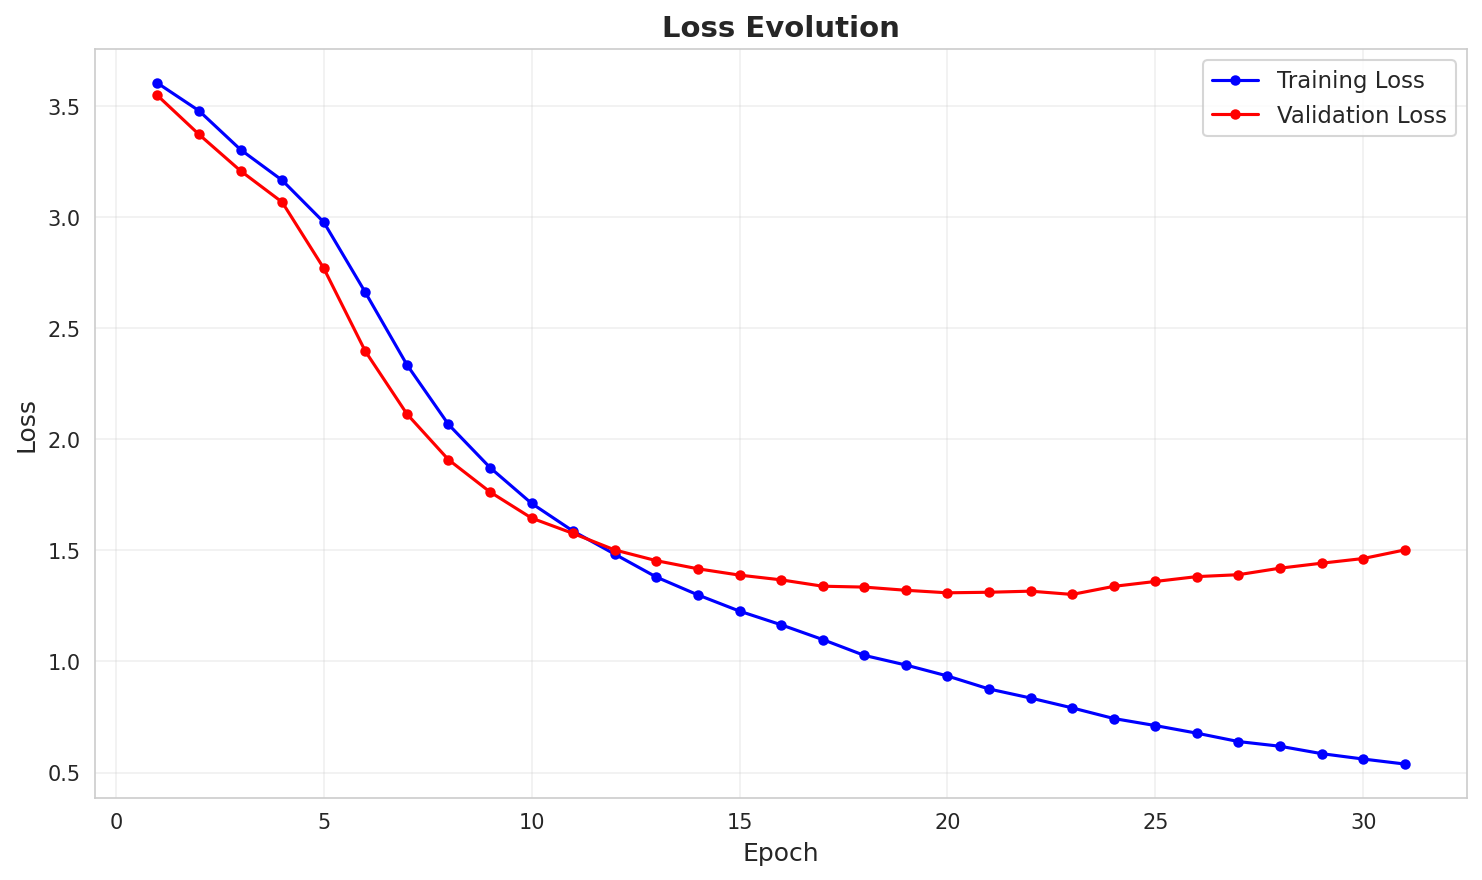
\includegraphics[width=0.90\textwidth]{loss_evolution.png}
  \caption{Training and validation loss curves for the optimized pipeline. The
  rapid initial decrease reflects effective warm-up and the benefit of the
  pre-trained backbone. The growing train/validation gap after epoch~10 is a
  controlled overfitting effect, mitigated by balanced class weighting, encoder
  freezing, and multi-sample dropout. The model was selected at the epoch of
  best Macro-F1.}
  \label{fig:loss}
\end{figure*}

\begin{figure*}[t]
  \centering
  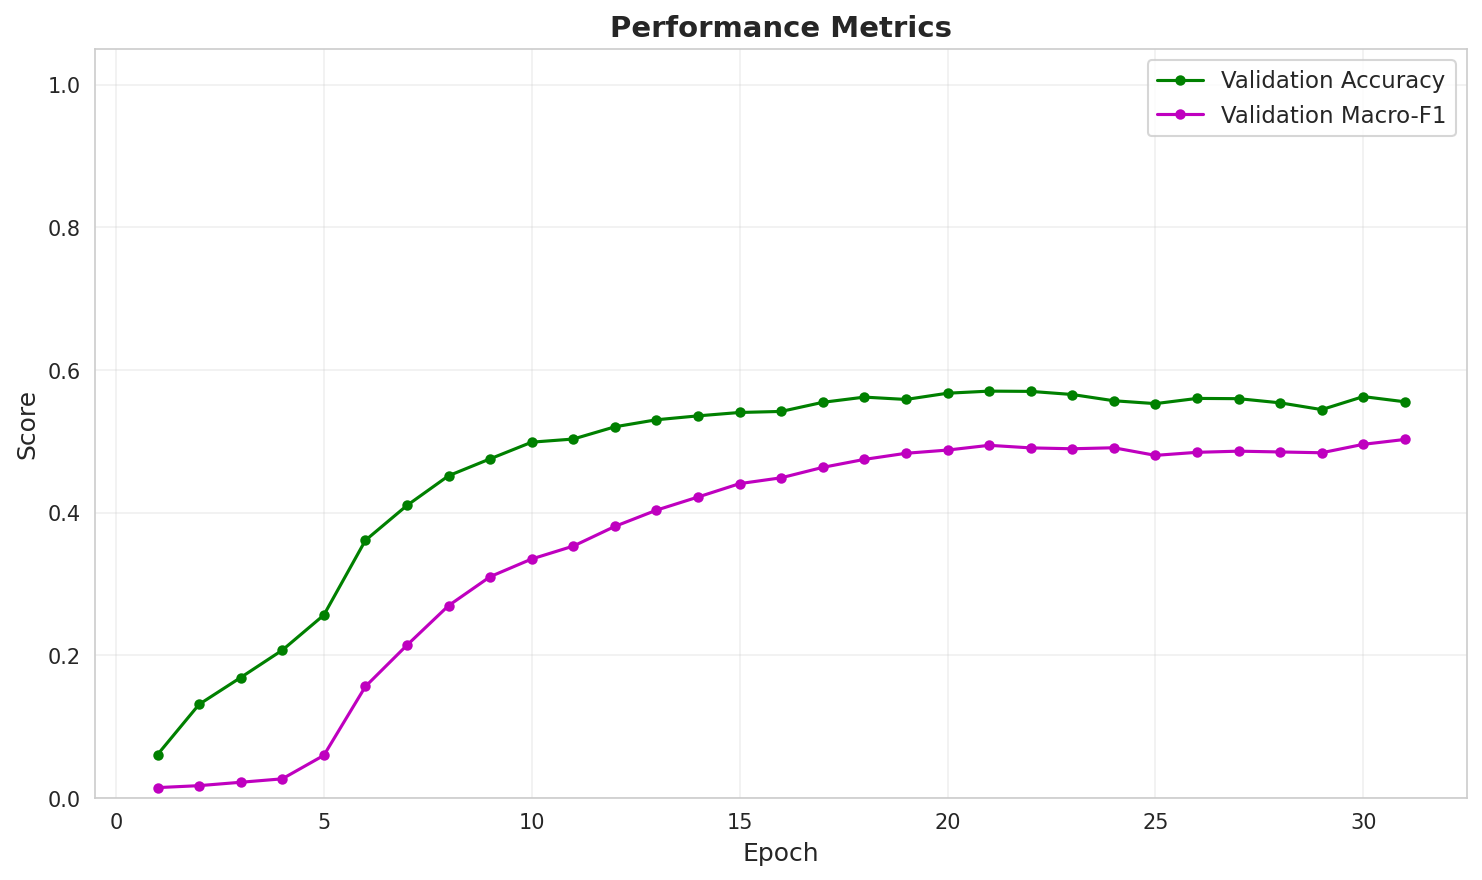
\includegraphics[width=0.90\textwidth]{performance_metrics.png}
  \caption{Validation accuracy and Macro-F1 over training epochs. Both metrics
  improve rapidly in the first 10--15 epochs as the model learns to distinguish
  major clinical categories. The Macro-F1 converges more slowly than accuracy
  because rare classes require more exposure to augmented dictionary samples.
  Early stopping is triggered when Macro-F1 plateaus, preventing the model from
  overfitting on the majority classes at the expense of rare-class performance.}
  \label{fig:perf}
\end{figure*}

\subsection{Analysis of Results}

\subsubsection{Successes of the Optimized Model}

\begin{itemize}
  \item \textbf{Generalization to Rare Diagnoses.} The combination of balanced
        class weights and ICD dictionary augmentation enabled the model to
        correctly identify rare long-tail categories (e.g.\ \texttt{U}, \texttt{W},
        \texttt{V}) that had near-zero recall in the baseline models. This is
        reflected in the macro-F1 jump from 0.258 (baseline mean pooling) to
        0.718 (optimized model).

  \item \textbf{Disambiguation of Procedural vs.\ Diagnostic Contexts.} The
        model successfully learned to distinguish procedure codes (\texttt{0}--\texttt{9})
        from diagnostic codes (\texttt{A}--\texttt{Z}), even when the literal
        is ambiguous (e.g.\ \textit{``retirada de cat\'{e}ter''} is a procedure
        category \texttt{0} despite containing a clinical noun).

  \item \textbf{Robustness to Lexical Noise.} The attention pooling mechanism
        learned to downweight grammatical fillers and focus on core diagnostic
        terms, improving robustness to Catalan/Spanish code-switching present
        in the real clinical literals.
\end{itemize}

\subsubsection{Remaining Shortcomings}

\begin{itemize}
  \item \textbf{Ultra-Short Literal Ambiguity.} Single-abbreviation literals such
        as \texttt{ia} cannot be disambiguated without broader patient context:
        it could represent \textit{Insufici\`encia A\`ortica} (category \texttt{I}),
        \textit{Inseminaci\'{o} Artificial} (category \texttt{Z}), or
        \textit{Insufici\`encia Arterial} (category \texttt{I}). The model tends
        to default to the maternity-biased class \texttt{O} or the procedure class
        \texttt{0} in these cases.

  \item \textbf{Granular Boundary Confusion.} The model occasionally confuses
        closely related ICD-10 chapters, such as endocrine disorders
        (\texttt{E}) vs.\ general symptoms (\texttt{R}). For example, the
        literal \textit{``Deshidrataci\'{o}n hipernattr\'{e}mica''} was sometimes
        misclassified as a general symptom (\texttt{R}) instead of a metabolic
        disorder (\texttt{E}).

  \item \textbf{Domain Mismatch in Augmentation.} The formal ICD-10 dictionary
        entries (averaging 35 words in structured medical Spanish) differ
        substantially in vocabulary and length from the real clinical literals
        (2--3 words, often abbreviated). This mismatch limits the benefit
        of augmentation for the most colloquial categories.
\end{itemize}

% ============================================================
\section{Conclusions and Future Work}
\label{sec:conclusion}
% ============================================================

\subsection{Summary of Contributions}

This project successfully designed, implemented, and evaluated an end-to-end
deep learning pipeline for automated Spanish ICD-10 codification. Key
contributions include:

\begin{enumerate}
  \item A \textbf{custom Attention Pooling} mechanism that outperforms both
        CLS and Mean pooling for short clinical literals by learning to focus
        on clinically informative subword tokens.
  \item A \textbf{Multi-Sample Dropout} regularization scheme that provides
        implicit ensembling within a single forward pass, reducing overfitting
        on the small primary clinical dataset.
  \item A rigorous \textbf{Split-Before-Augment} data engineering protocol that
        prevents data leakage from the ICD-10 dictionary augmentation and
        ensures reliable evaluation metrics.
  \item A comprehensive \textbf{training regularization stack} combining encoder
        layer freezing, balanced class-weight cross-entropy, cosine LR with
        warmup, gradient clipping, and AMP, enabling stable training on
        consumer-grade GPU hardware.
\end{enumerate}

The final optimized pipeline achieved \textbf{79.2\%} accuracy on the Kaggle
public leaderboard --- a relative gain of $+41.8\%$ over the baseline --- and
\textbf{71.8\%} Macro-F1 on the internal validation set, a gain of $+178\%$
over the baseline mean-pooling model.

\subsection{Future Work}

Several directions offer promising improvements beyond the current system:

\begin{itemize}
  \item \textbf{Synonym-based Data Augmentation.} Using medical terminology
        databases (e.g.\ SNOMED-CT, UMLS) to generate additional training
        paraphrases for rare categories.

  \item \textbf{Ensemble Methods.} Averaging predictions from multiple
        fine-tuned checkpoints or from models with different random seeds
        consistently improves robustness in NLP competitions.

  \item \textbf{Hierarchical Loss Functions.} Exploiting the tree structure of
        ICD-10 via hierarchical cross-entropy or label smoothing informed by
        taxonomic distance.

  \item \textbf{Contrastive Learning.} Pre-training the classification head
        with contrastive objectives (e.g.\ SimCSE [14]) on clinical literal pairs
        from the same ICD category to build tighter within-class representations.

  \item \textbf{Retrieval-Augmented Classification.} For ambiguous literals, a
        retrieval module could find the most similar labeled training examples
        and use their labels as additional context, implementing a nearest-neighbor
        correction step.
\end{itemize}

\subsection{Engineering and Ethical Takeaways}

\paragraph{Engineering.}
This project demonstrated that brute-force scaling of deep learning models is
suboptimal under real-world constraints. The three most impactful engineering
decisions were: (1) maintaining a leak-free validation split before augmentation;
(2) switching the early-stopping criterion from accuracy to macro-F1; and (3)
replacing the default single dropout with multi-sample dropout. Each of these
changes had a larger impact than simply training for more epochs.

\paragraph{Ethics.}
Deploying machine learning models in clinical environments carries significant
responsibility. The training data is heavily biased toward common hospital
encounters in a specific Catalan hospital system. A model trained on this data
may underperform for patients from underrepresented demographics or for rare
medical conditions not well represented in the training distribution. Any
production deployment would require bias auditing across subpopulations,
continuous monitoring of prediction quality, and mandatory human-in-the-loop
review for low-confidence predictions.

% ============================================================
% References (manual bibliography)
% ============================================================
\begin{thebibliography}{14}

\bibitem{yan2022}
C.\ Yan, X.\ Fu, X.\ Liu, Y.\ Zhang, Y.\ Gao, J.\ Wu, Q.\ Li,
``A survey of automated International Classification of Diseases coding:
development, challenges, and applications,''
\textit{Intelligent Medicine}, vol.~2, pp.~161--173, 2022.

\bibitem{taskspec}
E.\ Valveny, L.\ Kang,
``NLP-I Task: ICD-10 Codification --- Deep Learning Baseline,''
UAB Course Material, May 2026.

\bibitem{farkas}
R.\ Farkas, G.\ Szarvas,
``Automatic construction of rule-based ICD-9-CM coding systems,''
\textit{BMC Bioinformatics}, vol.~9 (suppl.~3), 2008.

\bibitem{perotte}
A.\ Perotte, R.\ Pivovarov, K.\ Natarajan, N.\ Weiskopf, F.\ Wood, N.\ Elhadad,
``Diagnosis code assignment: models and evaluation metrics,''
\textit{Journal of the American Medical Informatics Association}, vol.~21, no.~2,
pp.~231--237, 2014.

\bibitem{mullenbach}
J.\ Mullenbach, S.\ Wiegreffe, J.\ Duke, J.\ Sun, J.\ Eisenstein,
``Explainable prediction of medical codes from clinical text,''
\textit{Proc.\ NAACL-HLT}, pp.~1101--1111, 2018.

\bibitem{baumel}
T.\ Baumel, J.\ Nassour-Kassis, R.\ Cohen, M.\ Elhadad, N.\ Elhadad,
``Multi-label classification of patient notes: case study on ICD code assignment,''
\textit{Proc.\ AAAI Workshop on Health Intelligence}, 2018.

\bibitem{lee}
J.\ Lee, W.\ Yoon, S.\ Kim et al.,
``BioBERT: a pre-trained biomedical language representation model for
biomedical text mining,''
\textit{Bioinformatics}, vol.~36, no.~4, pp.~1234--1240, 2020.

\bibitem{alsentzer}
E.\ Alsentzer, J.\ Murphy, W.\ Boag et al.,
``Publicly available clinical BERT embeddings,''
\textit{Proc.\ Clinical NLP Workshop @ NAACL}, pp.~72--78, 2019.

\bibitem{vu}
T.\ Vu, D.\ Nguyen, A.\ Nguyen,
``Label attention model for ICD coding from clinical text,''
\textit{Proc.\ IJCAI}, pp.~3335--3341, 2021.

\bibitem{codiesp}
A.\ Miranda-Escalada et al.,
``Overview of automatic clinical coding at CodiEsp track of eHealth CLEF 2020,''
\textit{CLEF 2020 Working Notes}, 2020.

\bibitem{roberta}
Y.\ Liu, M.\ Ott, N.\ Goyal et al.,
``RoBERTa: A robustly optimized BERT pretraining approach,''
\textit{arXiv preprint}, arXiv:1907.11692, 2019.

\bibitem{adamw}
I.\ Loshchilov, F.\ Hutter,
``Decoupled weight decay regularization,''
\textit{Proc.\ ICLR}, 2019.

\bibitem{largebatch}
N.\ S.\ Keskar, D.\ Mudigere, J.\ Nocedal, M.\ Smelyanskiy, P.\ T.\ P.\ Tang,
``On large-batch training for deep learning: generalization gap and sharp minima,''
\textit{Proc.\ ICLR}, 2017.

\bibitem{simcse}
T.\ Gao, X.\ Yao, D.\ Chen,
``SimCSE: Simple Contrastive Learning of Sentence Embeddings,''
\textit{Proc.\ EMNLP}, pp.~6894--6910, 2021.

\end{thebibliography}

\end{document}
